\chapter[Introdução]{Introdução}

Este documento é definido como um conjunto de pesquisas e descri\c{c}\~oes de atividades que ir\~ao resultar em um projeto de melhorias que utilizam exclusivamente solu\c{c}\~oes tecnol\'ogicas para o Parque Urbano do Gama-DF. Esse projeto deve ser detalhado de modo a ser poss\'ivel uma futura utiliza\c{c}\~ao das ideias aqui descritas atrav\'es de simula\c{c}\~oes, esquem\'aticos e texto descritivo. 

\section{Contextualiza\c{c}\~ao}

O Parque Vivencial do Gama localiza-se na Regi\~ao Administrativa II do Gama, criada atrav\'es da Lei n.$^o$ 49/89 e do Decreto n.$^o$ 11.921/89 e formada por \'area urbana e rural. A \'area urbana \'e dividida em seis setores, sendo: Norte, Sul, Leste, Oeste, Central e de Ind\'ustria. O Parque Vivencial do Gama est\'a localizado no setor Norte (coordenadas 16 $^o$ 00`13.4``S 48 $^o$03`55.0``W), ocupando uma \'area de aproximadamente 52 mil m$^{2}$ \cite{COEX}. A Figura abaixo apresenta a imagem da \'area do parque.

\begin{figure}[h]
	\centering
	\label{Imagem do Parque Vivencial do Gama}
		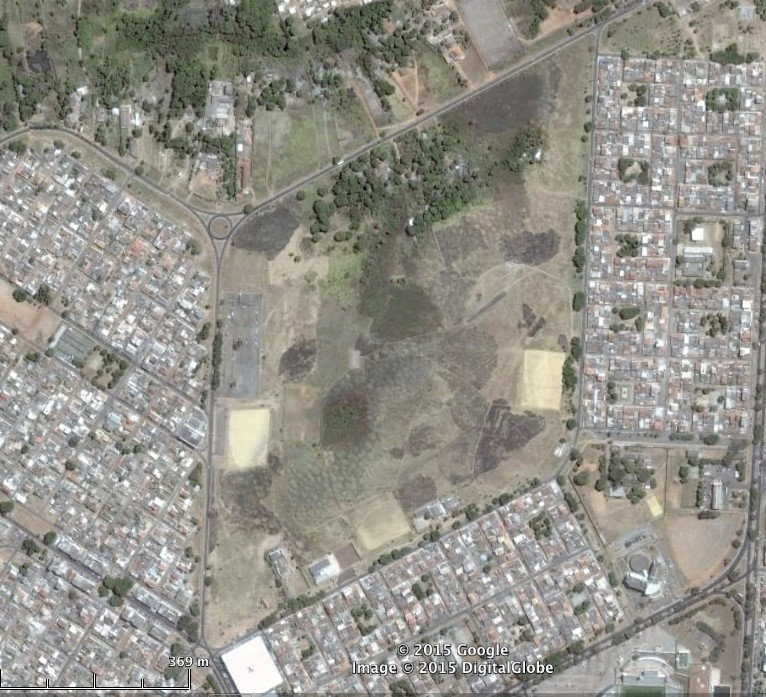
\includegraphics[keepaspectratio=true,scale=0.6]{figuras/ParqueVivencialGama.jpg}
	\caption{Imagem do Parque Vivencial do Gama}
	\small{Fonte: Google, 2015}
\end{figure}

A vegeta\c{c}\~ao que existente no Parque est\'a ligada ao Bioma Cerrado, mas no momento n\~ao se encontra preservado restando apenas esp\'ecies do tipo buritis, pata-de-vaca (Bauhinia variegata) e vegeta\c{c}\~ao rasteira.  O solo do parque \'e hidrom\'orfico, ou seja, tem excesso de umidade. Nessa \'area tamb\'em h\'a nascentes o que limita a constru\c{c}\~ao civil no pr\'oprio parque perante a Lei N$^{o}$ 12.651/12 - C\'odigo Florestal, a qual prev\^e prote\c{c}\~ao \`a \'area de nascentes. Abaixo, tem-se as figuras abaixo apresentam respectivamente, a vegeta\c{c}\~ao e as nascentes \cite{COEX}.

\begin{figure}[h]
	\centering
	\label{Imagem do Parque Vivencial do Gama}
		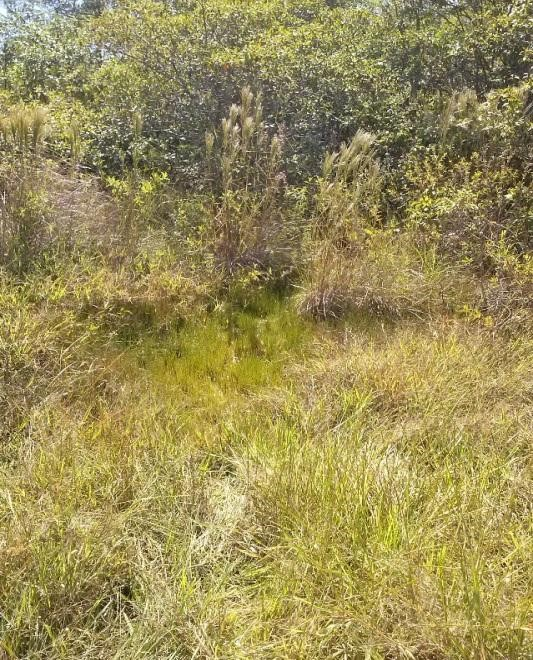
\includegraphics[keepaspectratio=true,scale=0.4]{figuras/VegatacaoTipica.jpg}
	\caption{Imagem da vegata\c{c}\~ao T\'ipica.}
	\small{Fonte: Administra\c{c}\~ao do Gama, 2015}
\end{figure}

\begin{figure}[h]
	\centering
	\label{Imagem do Parque Vivencial do Gama}
		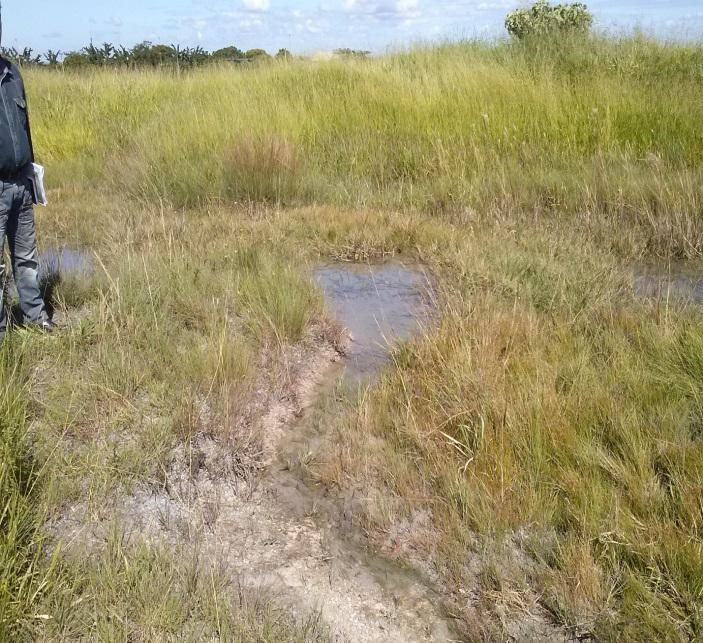
\includegraphics[keepaspectratio=true,scale=0.4]{figuras/Nascentes.jpg}
	\caption{Imagem de uma das nascentes.}
	\small{Fonte: Administra\c{c}\~ao do Gama, 2015}
\end{figure}

Inicialmente o Parque Vivencial do Gama foi projetado com uma infraestrutura que possu\'ia \textit{playground}, quadras poliesportivas, pistas de \textit{cooper} e ciclovia, espa\c{c}os de conviv\^encia, entre outros aparatos \cite{Ibram}. Al\'em disso, possui tamb\'em banheiros, quiosques, quatro campos de futebol e o pr\'edio da administra\c{c}\~ao. Mas, segundo integrantes do grupo que visitaram o parque, todos esses itens est\~ao em p\'essimas condi\c{c}\~oes de conservamento e de uso ou est\~ao sendo usados para outros fins, como por exemplo, o \textit{playground} que \'e usado por usu\'arios de drogas como um local de conviv\^encia. 

\section{Descri\c{c}\~ao do problema}

\begin{figure}[H]
	\centering
	\label{FISHBONE}
		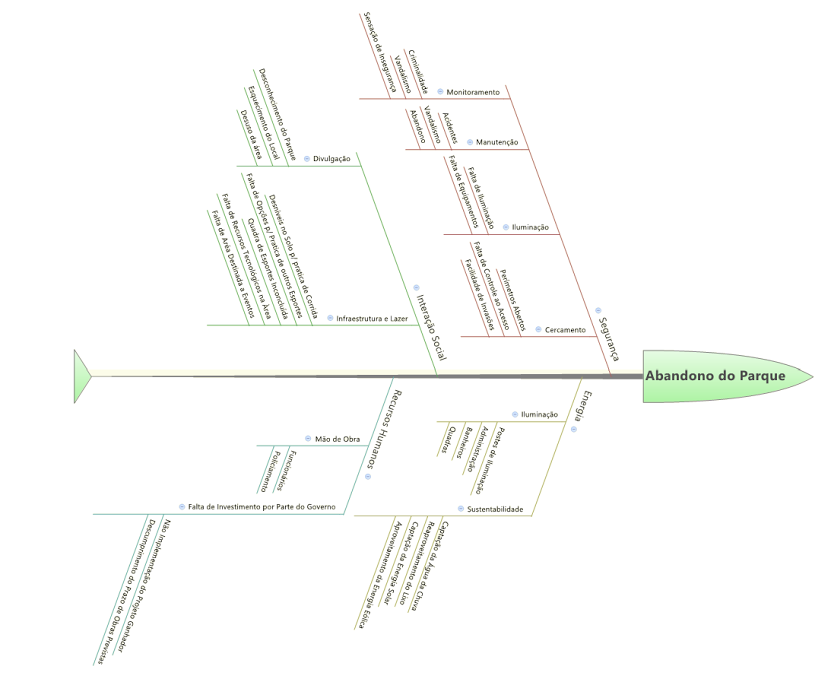
\includegraphics[keepaspectratio=true,scale=0.6]{figuras/FISHBONE_complete.png}
	\caption{Fishbone do projeto.}
\end{figure}

Os problemas apresentados s\~ao descridos a seguir:

\subsection{Problemas encontrados}
\subsubsection{Ilumina\c{c}\~ao}

A ilumina\c{c}\~ao \'e um dos grandes problemas do parque. Sem uma ilumina\c{c}\~ao adequada a sensa\c{c}\~ao de seguran\c{c}a \'e m\'inima, dando condi\c{c}\~oes propicias ao crime e consequentemente diminuindo o n\'umero de frequentadores do parque.

\subsubsection{Falta de Monitoramento do Parque}

O monitoramento do parque \'e quase nulo, muitos lugares estão sendo usados para pr\'aticas de crimes, passando a sensa\c{c}\~ao de abandono do parque com consequ\^encias similares a da falta de ilumina\c{c}\~ao, um bom monitoramento resolveria os problemas do parque, como tamb\'em o da popula\c{c}\~ao das imedia\c{c}\~oes da \'area patrulhada.

\subsubsection{Danos na cerca do parque}

O cercamento do parque est\'a em condi\c{c}\~oes medianas de conserva\c{c}\~ao, mas possui buracos e em algumas \'areas ele \'e ausente propiciando invas\~oes do terreno, crimes, esconderijos para criminosos e degrada\c{c}\~ao ambiental.

\subsubsection{Falta de manuten\c{c}\~ao da infraestrutura}

A manuten\c{c}\~ao do parque \'e prec\'aria, com brinquedos quebrados, cal\c{c}adas rachadas al\'em de problemas com a ilumina\c{c}\~ao, isso causa acidentes, evita a pr\'atica de esportes e prejudica o lazer. Solucionando este problema o parque ficaria em boas condi\c{c}\~oes para e uso, evitando reformula\c{c}\~oes do projeto, conservando assim o dinheiro e protegendo a fauna e flora local. 

\subsubsection{Fonte n\~ao sustent\'avel de energia}

N\~ao existe uma fonte sustent\'avel de fornecimento de energia para o parque.

\subsubsection{Lixo produzido nos banheiros por usu\'arios e pela administra\c{c}\~ao}

O lixo produzido deve ter uma devida destina\c{c}\~ao para n\~ao danificar o local. Este fator \'e extremamente importante, uma vez que o parque \'e considerado reserva ambiental.

\subsubsection{A falta de atratividade do parque}

A falta de atratividade do parque devido \`a falta de op\c{c}\~ao de recrea\c{c}\~ao, falta de intera\c{c}\~ao entre as pessoas, al\'em de todos os problemas estruturais b\'asicos.

\subsection{Quem s\~ao os afetados pelos problemas encontrados}

Os problemas listados podem afetar diretamente ou indiretamente v\'arios p\'ublicos, dentre eles est\~ao a comunidade vizinha ao parque, as crian\c{c}as e jovens que estudam em escolas pr\'oximas. Pessoas que procuram um local para praticar esportes ao ar livre e ter op\c{c}\~oes de lazer e intera\c{c}\~ao social.
	Outro grupo que possivelmente frequenta o parque s\~ao os moradores de rua e habitantes de moradias n\~ao regulamentadas. Sendo assim, policiais, ONG's e agentes governamentais necessitar\~ao estarem presentes.
	Al\'em de toda a comunidade ao redor do parque, que n\~ao necessariamente seja composta apenas por moradores. Incluindo comerciantes, universit\'arios, funcion\'arios do setor p\'ublico em geral que busquem um local de lazer para a os intervalos de trabalho e o fim do expediente.
	Contudo, o local tamb\'em \'e apropriado para receber eventos a n\'ivel distrital devido a sua representatividade e ao espa\c{c}o dispon\'ivel. Afirmando sua caracter\'istica sustent\'avel e ecol\'ogica, o parque buscar\'a repercutir e atrair cada vez mais pessoas.
	
\subsection{Impactos}

Todo problema gera impactos e \'e necess\'ario identificar cada um deles para poder priorizar solu\c{c}\~oes para as causas mais graves. Em seguida s\~ao apresentados impactos observados com o abandono do Parque Urbano do Gama e seus problemas decorrentes:

\begin{itemize}
	\item N\~ao aproveitamento do potencial de atividades que o parque pode oferecer;
	\item A popula\c{c}\~ao n\~ao possui responsabilidade em cuidar, cobrar as autoridades locais;
	\item Ambiental: na forma de polui\c{c}\~ao visual, degrada\c{c}\~ao ambiental, solo, len\c{c}ol fre\'atico;
	\item Presen\c{c}a de usu\'arios de entorpecentes;
	\item Inseguran\c{c}a;
	\item Crimes nas redondezas;
	\item Degrada\c{c}\~ao do patrim\^onio p\'ublico;
	\item Degrada\c{c}\~ao ambiental;
	\item Acidentes;
\end{itemize}

\section{Justificativa}

A principal motiva\c{c}\~ao do projeto consiste no abandono do parque pela popula\c{c}\~ao e pelo governo, resultando na falta de aproveitamento do parque, em seu potencial social, ecológico e turístico. Com a devida revitaliza\c{c}\~ao, o parque poderia acrescentar op\c{c}\~oes de intera\c{c}\~ao social para o Gama, favorecendo os moradores da cidade e a todos que possam frequent\'a-la.
Devido a essa motiva\c{c}\~ao o que se encontra na realidade do parque s\~ao problemas de seguran\c{c}a, limpeza, o que acarreta baixa especula\c{c}\~ao imobili\'aria em torno e invas\~oes. 

\section{5W2H}

A primeira atividade realizada pelo grupo foi responder o 5W2H para ter no\c{c}\~oes iniciais das motiva\c{c}\~oes, causas entre outras informa\c{c}\~oes relacionadas ao projeto. A seguir est\~ao as respostas estabelecidas pelo grupo.

\subsection{What? (O que ser\'a entregue?)}

Ser\'a entregue um projeto de revitaliza\c{c}\~ao de um parque urbano, em que ser\'a utilizada a tecnologia como principal ferramenta.

\subsection{Why? (Por qu\^e est\'a sendo feito?)}

Est\'a sendo realizado devido a atual inutiliza\c{c}\~ao de um espa\c{c}o p\'ublico que possui grande potencial de servir a comunidade vizinha, com o prop\'osito de uma maior comodidade e incentivo ao acesso a partir das aplica\c{c}\~oes tecnol\'ogicas, o que seria um diferencial em vista de outros parques.

\subsection{Where? (Onde ser\'a feito/ entregue/ utilizado?)}

Ser\'a feito no parque vivencial urbano localizado na cidade do Gama do Distrito Federal. Uma regi\~ao de cerrado, n\~ao preservado, em que h\'a invas\~oes ilegais, pista de aeromodelismo, problemas de seguran\c{c}a e limpeza.

\subsection{When? (Quando ser\'a feito/ entregue?)}

O projeto tem dura\c{c}\~ao de tr\^es meses, tendo como data final de entrega dia 22 de junho de 2015.

\subsection{Who? (Quem o far\'a?)}

A realiza\c{c}\~ao deste projeto ser\'a pelos alunos de gradua\c{c}\~ao dos cursos de Engenharia conciliada com empresas interessadas, o Governo do Distrito Federal, \textit{stakeholders} em geral, como a popula\c{c}\~ao interessada.

\subsection{How? (Como ser\'a realizado?)}

Ser\'a realizado a partir de pesquisas acerca do tema, reuni\~oes, debates de ideias e utiliza\c{c}\~ao de metodologias de gerenciamento de projetos, como o \textit{SCRUM} e ferramentas de comunica\c{c}\~ao, como o \textit{Trello}.

\subsection{How much? (Quanto custar\'a?)}

Analisando, primeiramente a hora-homens trabalhadas, pode-se estimular um valor.

Determinando: 
\begin{itemize}
        \item 9 pessoas ganhando 6 mil
	\item 8 pessoas ganhando 9 mil
	\item 8 pessoas ganhando 4 mil
\end{itemize}

semanalmente 8 horas trabalhadas --- um m\^es 32 horas
acrescentando 25\% de risco

Tem-se : R\$ 197500,00 o que corresponde em hora/m\^es a R\$ 246,32.

\section{Objetivos}

Nesta se\c{c}\~ao est\~ao descritos os objetivos que devem ser atingidos ao final deste projeto.

\subsection{Objetivo Geral}

Buscar solu\c{c}\~oes tecnol\'ogicas para aumentar a atratividade do parque urbano e vivencial do Gama - DF, aumentando a intera\c{c}\~ao social por parte da popula\c{c}\~ao, fornecendo lazer, sustentabilidade, seguran\c{c}a e preservando a natureza do local. 

\subsection{Objetivos Espec\'{\i}ficos}

Integrar os cursos de engenharia: automotiva; aeroespacial; energia; eletr\^onica e software em que situam os alunos a projetar, colocar em pr\'atica conceitos estudados. 
Apresentar um planejamento de como executar a revitaliza\c{c}\~ao tecnol\'ogica. Relacionar os aspectos f\'isicos e burocr\'aticos que se encontram na regi\~ao atualmente, e as obras j\'a iniciadas pela Administra\c{c}\~ao Regional do Gama; com as legisla\c{c}\~oes distritais que limitam no tocante ao meio ambiente, a popula\c{c}\~ao vizinha e os impactos urbanos. 

\section{Metodologia}

\subsection{Estrutura Organizacional}

O grupo foi subdividido em grupos menores visando resolver os principais problemas encontrados no parque.

\begin{figure}[H]
	\centering
	\label{Estrutura Organizacional}
		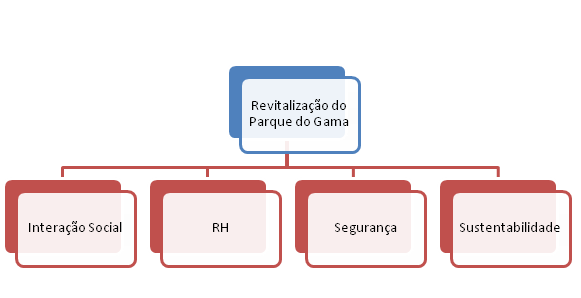
\includegraphics[keepaspectratio=true,scale=1.0]{figuras/EstruturaOrganizacional.png}
	\caption{Esquem\'atico da divis\~ao dos grupos do projeto.}
\end{figure}

\begin{itemize}
    \item Sustentabilidade: Esse grupo visa a sustentabilidade do parque, preocupando-se com as quest\~oes ambientais.
	\item Seguran\c{c}a: Esse grupo visa tornar o ambiente seguro para visita\c{c}\~ao.
	\item Recursos Humanos - Controle: Esse grupo visa administrar os entreg\'aveis, organiza a documenta\c{c}\~ao, controla a integra\c{c}\~ao de todo o grupo.
	\item Interação social: Esse grupo visa tornar o parque mais atrativo de forma que possa interrelacionar a população do Gama e região.
\end{itemize}

\subsection{Gerenciamento dos Recursos Humanos}

Esta se\c{c}\~ao mostra como os integrantes do projeto foram alocados e quais as suas respectivas fun\c{c}\~oes.

\subsubsection{Pap\'eis e Responsabilidades}
Esta subse\c{c}\~ao mostra os pap\'eis dos integrantes do projeto e quais as suas respectivas responsabilidades.

\begin{table}[H]
\caption{Descri\c{c}\~ao das atividades de cada um dos membros.} 
\begin{center}
\begin{tabular}{|p{3cm}|p{4cm}|p{8cm}|} \hline

Cargo &Nome &Fun\c{c}\~ao\\ \hline 

Gerente Geral &Let\'icia Barros &Planejar atividades coletivas, bem como estabelecer t\'opicos de discuss\~ao para as reuni\~oes presenciais. Al\'em disso, deve acompanhar o desenvolvimento dos subgrupos e buscar a integra\c{c}\~ao entre eles para que todos possam seguir processos espec\'ificos que devem se interrelacionar ao longo do projeto buscando um melhor desempenho geral \\ \hline

Subgerentes &Let\'icia Munhoz (Intera\c{c}\~ao Social)  Helton (Seguran\c{c}a)  Renner (Sustentabilidade)  Ebenezer (RH) &Planejar reuni\~oes menores para cada um dos seus grupos, designar tarefas para cada um dos seus membros e averiguar a qualidade dos artefatos, no tempo esperado e repassar essas informa\c{c}\~oes para que a gerente geral e os demais alunos possam acompanhar o que est\'a sendo feito \\ \hline

Pesquisadores de sustentabilidade &Lucas Rossi, Henrique, Daniel, Matheus Coelho, Bernardo &Trabalhar de forma a encontrar as solu\c{c}\~oes mais vi\'aveis para gerar energia para as atividades do parque sem desrespeitar a legisla\c{c}\~ao vigente \\ \hline
Pesquisadores de Intera\c{c}\~ao Social &Eduardo, Fernanda, Diogo, Ruan e Rodrigo &Realizar o acompanhamento da popula\c{c}\~ao do Gama e poss\'iveis interessados na reforma do parque para buscar formas de aumentar a atratividade do local \\ \hline 

Pesquisadores de seguran\c{c}a &Divino, Matheus Alves, David, Higor, Victor Hugo, Victor Henrique &Projetar mecanismos para controlar a seguran\c{c}a do parque de forma a oferecer um ambiente seguro para visita\c{c}\~ao \\ \hline

Pesquisadores de controle &Luciana, Lu\'is e Marcos Gois. &Esse grupo visa administrar os entreg\'aveis, organiza a documenta\c{c}\~ao, controla a integra\c{c}\~ao de todo o grupo. \\ \hline

 \end{tabular}
\end{center}
\end{table}

\subsection{Plano de Comunica\c{c}\~ao}

Para a comunica\c{c}\~ao foram utilizadas v\'arias plataformas, como descrito a seguir:
\\ \\ \textit {Facebook}: foi a primeira ferramenta utilizada e o grupo foi criado na primeira reuni\~ao do projeto. Inicialmente documentos eram compartilhados utilizando essa ferramenta, o que n\~ao se mostrou muito eficaz pela falta de recursos para organizar os arquivos e pelo site ser bloqueado na Universidade. No entanto, a ferramenta ainda \'e utilizada para avisos r\'apidos sobre atividades. 
\\ \textit{Whatsapp}: esta ferramenta foi utilizada para aumentar o n\'ivel de intera\c{c}\~ao dos membros e tamb\'em serve para avisos gerais, como comunicar que alguma documenta\c{c}\~ao deve ser atualizada.
\\ \textit{Google Drive}: ferramenta mais utilizada pelo grupo. Ela serve como banco de dados. Todas as refer\^encias e resultados de pesquisas tem sua documenta\c{c}\~ao organizada nessa plataforma. Ela se mostrou atrativa por poder ser melhor organizada, oferecer um grande espa\c{c}o de mem\'oria e possibilidade de edi\c{c}\~ao de documentos em grupo.
\\ \textit{Trello}: esta ferramenta foi utilizada com o \'unico intuito de ser um local de acesso r\'apido para a averigua\c{c}\~ao do andamento das atividades propostas.

\begin{figure}[H]
	\centering
	\label{comunicacao}
		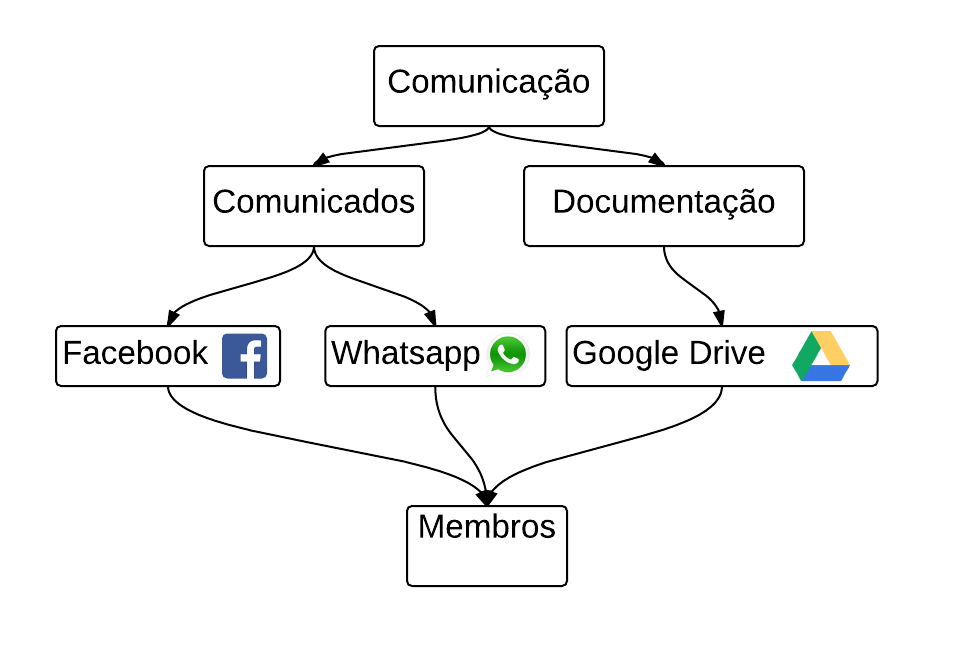
\includegraphics[keepaspectratio=true,scale=0.7]{figuras/comunicacao.png}
	\caption{Esquem\'atico de comunica\c{c}\~ao}
\end{figure}

\subsection{Gerenciamento do Tempo}

A gest\~ao do tempo partiu das datas dos Pontos de Controle (PC1, PC2 e PC3), Atrav\'es dessas datas foram estipulados os pontos cr\'iticos de entregas do projeto. Para relacionar as atividades fundamentais a serem realizadas pela equipe foi feita uma rela\c{c}\~ao entre as atividades da metodologia, que \'e descrita na pr\'oxima se\c{c}\~ao e os entreg\'aveis da EAP (Estrutura Anal\'itica de Projeto).
Os prazos para realiza\c{c}\~ao das atividades iniciais foram realizados de acordo com as necessidades do projeto, como constru\c{c}\~ao de artefatos e realiza\c{c}\~ao de tarefas. 
A partir da sprint 0 foi abordado o prazo para realiza\c{c}\~ao da sprint entre os subgerentes e a gerente de projeto que foi definido de uma semana. Essa sprint ser\'a a sprint modelo para que se possa tomar conhecimento da real necessidade de tempo que a equipe levar\'a para realizar as atividades demandadas. Com base nessas informa\c{c}\~oes foi constru\'ido no final da macro atividade - Manter Planejamento - a primeira vers\~ao do cronograma. A primeira vers\~ao do documento segue em anexo no final do relat\'orio .

\subsection{Desenvolvimento de Projeto/ Metodologia}

Para selecionar uma metodologia para apoiar o desenvolvimento foi analisado o ambiente do projeto, rela\c{c}\~ao entre a parte interna da equipe, rela\c{c}\~ao entre equipe e cliente e o impacto sobre os \textit{stakeholders}. 
	O projeto apresenta requisitos inst\'aveis, tamb\'em como o surgimento de novos requisitos durante a execu\c{c}\~ao do projeto, essas caracter\'isticas s\~ao uma das que mais impactaram a sele\c{c}\~ao da metodologia \textit{Scrum}. Tamb\'em o contato com o cliente ocorre de forma simples e pode ser estabelecida semanalmente. O cliente identificado na identifica\c{c}\~ao dos \textit{stakeholders} \'e a Administra\c{c}\~ao do Gama-DF e devido a proximidade geogr\'afica de alguns integrantes da equipe de desenvolvimento com a Administra\c{c}\~ao do Gama acabou influenciando a sele\c{c}\~ao da metodologia. 
Para adapta\c{c}\~ao da metodologia de acordo com as reais necessidades do projeto, primeiramente foi utilizado o SAFe (\textit{Scaled Agile Framework}) que fornece uma estrutura para aplica\c{c}\~ao de metodos \'ageis para desenvolvimento de projetos. A partir deste \textit{framework} foi constru\'ido um processo de desenvolvimento que ser\'a aplicado no projeto de acordo com as necessidades da equipe. O processo foi modelado utilizando o Bizagi Modeler, abaixo segue a descrição do processo modelado

\subsubsection{Visão Completa do Processo}
\begin{figure}[H]
	\centering
	\label{Visão geral do processo modelado}
		\includegraphics[keepaspectratio=true,scale=0.9,angle=270]{processo/ProcessoCompleto.png}
	\caption{Visão geral do processo modelado.}
\end{figure}

\subsubsection{Iniciar Projeto}

\begin{figure}[H]
	\centering
	\label{Visão do processo Iniciar Projeto}
		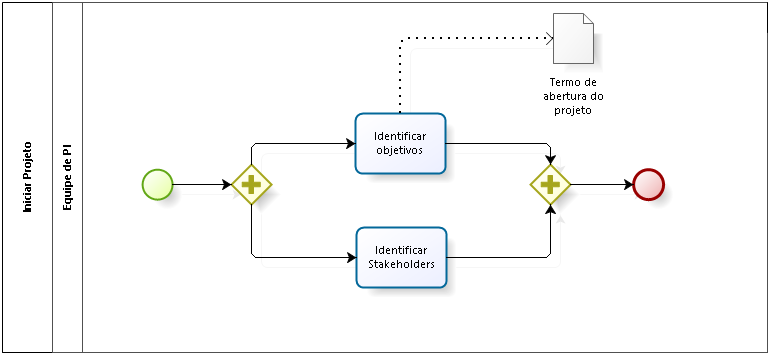
\includegraphics[keepaspectratio=true,scale=0.9,angle=270]{processo/IniciarProjeto.png}
	\caption{Visão do processo Iniciar Projeto.}
\end{figure}

No processo iniciar projeto é onde ocorre o levantamento das informações fundamentais para iniciação do projeto. 

\begin{enumerate}
	\item Identificar objetivos. 
		Identificar todos os objetivos necessários para realização do termo de abertura do projeto, é nessa atividade que esse artefato é construído.
	\item Identificar stakeholders.
		Identificar todas as pessoas e organizações que estão interessadas ou serão impactadas com o desenvolvimento do projeto. 
\end{enumerate}

\begin{itemize}
	\item Termo de abertura do projeto
	Documento com as definições fundamentais para definição/estruturação do trabalho. 
\end{itemize}

\section{Definição de Escopo do Projeto}

	O projeto consiste em desenvolver soluções tecnológicas para o parque do Urbano e Vivencial do Gama. Foi observado que o parque apresenta uma grande extensão, de aproximadamente 52 mil metros quadrados. No entanto, não se mostrou viável criar soluções que estejam presentes por toda a extensão do parque. A primeira restrição que foi adotada foi com relação ao processo que está em andamento por parte da Administração Regional. Através de visitas ao local foi possível obter a planta entre outras informações sobre o projeto implementado. Dessa forma, caso o projeto desenvolvido na disciplina de Projeto Integrador 1 se torne viável, seria interessante apresentá-lo para possíveis steakholders. 

	Dentro das delimitações do projeto estipulou-se um número de visitantes em dias de alta movimentação, como os fins de semana, em torno de 1300 pessoas. Este número foi embasado em uma comparação com o Parque de Águas Claras e uma combinação desse valor com o número de visitantes esperados devido ao espaço Lazer- Multimídia. 
Dentro dos subsistemas também foram estipuladas delimitações para o projeto. 
	
	O espaço de interação social está sendo projetado para suportar um número de até 1000 pessoas. Dentro deste espaço terão 30 bicicletas ergométricas. A energia gerada pelas mesmas será consumida simultaneamente, sem o armazenamento de energia. 
	
	A energia gerada pelos painéis fotovoltáicos será armazenada para alimentar os mesmos durante o período que a luz ambiente for menor, no geral no período noturno. Os outros equipamentos do parque, que não incluam a iluminação geral e nem o espaço interativo serão alimentados pela energia elétrica da rede, um consumo estimado em torno de  2054,57 kWh. A Segurança projetada para o parque tem foco na segurança das pessoas e patrimônio físico, não abrangendo a segurança ambiental. Consequentemente uma das soluções abordadas é o cercamento do parque. O perímetro estipulado para tal é de 3342,29 metros. 